\subsubsection{Gate-Treiber}
\label{subsubsec:Inbetriebnahme_Gate_Treiber}

Der Gate-Treiber wird ebenfalls über die SPI-Schnittstelle in Betrieb genommen. Dazu werden die Parameter verwendet, welche aus der TMCL-IDE verwendet werden. Die Standardparameter beinhalten Informationen zum Motor \todo{Kurz beschreiben, was die Register beinhalten} und Einschalten des Treibers.

\begin{figure}[h!]
\center
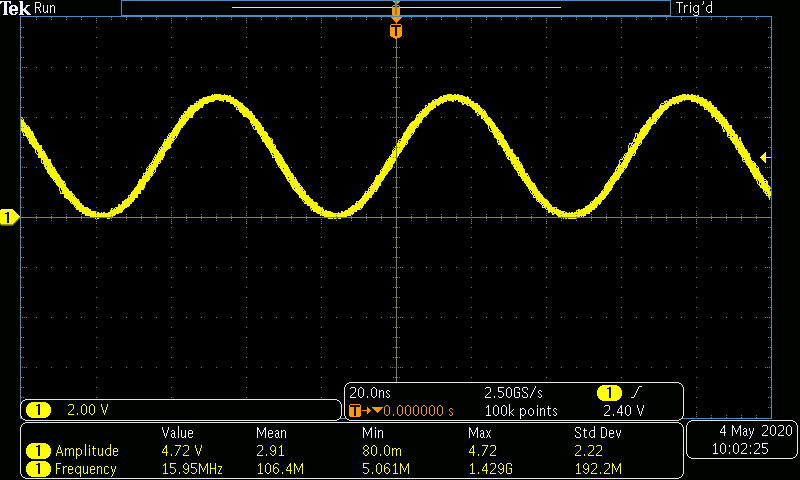
\includegraphics[width = 0.8\textwidth]{graphics/Crystal_Swing}
\caption{Schwingung des Oszillators}
\label{fig:Crystal_Swing}
\end{figure}

Die Initialisierung sowie das Auslesen gewisser Register ist mit der Testapplikation ''\textit{Motor}'' möglich. Auch die Initialisierung und Kommunikation mit den Gate-Treiber TMC4671 kann mit diesem getestet werden.

Vorgehen:
\begin{enumerate}
\item Benötigte Applikation aus dem Software-Ordner auf dem USB-Stick in Atmel Studio öffnen.\\
\textcolor{magenta}{Software\textrightarrow Atmega\textrightarrow 5\_Motor\textrightarrow Motor}\\

\item Software anpassen:\\
\textcolor{green}{
TMC6200\_init();\\
ggf. Pins, UART- und SPI-Schnittstelle\\
}
\item Software hochladen:\\
\textcolor{blue}{AtmelStudio\textrightarrow Tools\textrightarrow Cocktailmixer}\\

\item Ausgehende Gate-Signale auf den Gatevorwiderstand des MOSFETS mit Oszilloskop überprüfen.

\todo{Bilder machen und einfügen mit Oszi.}

\textcolor{red}{Fehler}\\
Hier ergibt sich ein Problem mit dem Ansteuern der H-Brücke. Der Gate-Treiber schaltet die Gatesignale des FOC-Treibers nicht wie gewünscht durch, sondern bleibt auf einem Schaltzustand stehen. Dies führt dazu, dass die MOSFETS die H-Brücke nicht schalten und der Motor nicht läuft. Die Belegung der Pins und Spannungslevel an den Konfigurationspins ist jeweils die Selbe wie beim EVAL-Kit.\\

Eine Möglichkeit besteht in der Beschaltung des externen Gate-Spannungs-Regulator. Im Datenblatt des TMC6200-TA steht auf Seite 11 geschrieben, dass die Verluste der internen Spannungsregler bei höheren Spannungen ab 48V mit einem externen Spannungsregler verringert werden können. Die sonstige Beschaltung ist gleich der von Trinamic.\\

Aus Zeitgründen wurde entschieden, dass zur Lösung das Universal Power Supply UPS-70V10A zum Einsatz kommt. Dieses wurde schon im P5 verwendet und ermöglicht ein Umgehen des Gate-Treibers, indem einfache Bauteile ohne komplizierte Logik verwendet werden. Dies hat den Vorteil, dass für die Ansteuerung des Motors nur die schon in Betrieb genommenen Gate-Signale des TMC4671 von Wichtigkeit sind. Für einen vorläufigen Betrieb läuft der Print also mit externer H-Brücke und Gate-Treiber.

\end{enumerate}